\documentclass[•]{article}
\usepackage{graphicx, float}
\usepackage{caption}
\usepackage{subcaption}
\usepackage{amsmath}

\author{Tijmen Wintjes}
\title{Lightsoccer}


\newcommand{\apicture}[2] {
  \begin{figure}[H]
  \centering
  \includegraphics[width=0.5\textwidth]{#1}
  \caption{#2}
  \end{figure}
  }

\begin{document}

\maketitle

\section{Formulation of the optimization problem}
This report treats the problem sketched the figure. A soccer player is approaching a the goal whilst the keeper tries to protect as much of the goal as possible. 

\apicture{soccer1.jpg}{Light soccer situation with keepe rat (2,10), attacker at (2,20) and the keeper 
being at an angle of $\pi/2$}
Given the position of the attacker we can calculate what the optimal 

Given that we know where the attacker will be, we should calculate the optimal position of the keeper. To find the optimum placement of the keeper we juse the fuction:
\begin{align*}
J &= x_l^2 + x_r^2
\end{align*}
Where $x_l$ and $x_r$ are respectively the left and right uncovered parts of the goal. In the picture above $x_l$ = 4.17 and $x_r$ = 0.02
\\\\
As small uncovered edges in the corners will lead to small costs, it is likely that the keeper will not fully cover a corner, but will rather choose to cover a bigger part of the other corner. In other words the keeper will stay more in the middle. This is okay, as it is hard for soccer player to aim precisely. 
\\\\
To get an idea of the costfunction a  3D plot was made. In the figure below a topview is presented. The white part in the picture is close to the attacker, too close such that a division by zero occurs in the calculation. This is okay as these values correspond with unfeasible points.

\apicture{costfunc.jpg}{A topview of the costfunction, theta = 0, the colors give the levels of the costfunction.}
The optimization problem to be solved is the following. W $maxx_k = 19.66$
\begin{align*}
\min\limits_{x_k,y_k,\theta} & J(x_k,y_k,\theta) \\
s.t. & -19.66 \leq x_k \leq 19.66 \\
&  0 \leq y_k \leq 16 \\
&  -\pi/2 \leq \theta \leq \pi/2 \\
\end{align*}

\section{Dynamic keeper model}
The symbolic expression of the discrete matrices Ad, Bd, Cd and Dd are displayed in the figure below. 

\begin{align*}
Ad &= \left(\begin{array}{cccccc} 1 & 0 & 0 & \mathrm{Ts} & 0 & 0\\ 0 & 1 & 0 & 0 & \mathrm{Ts} & 0\\ 0 & 0 & 1 & 0 & 0 & \mathrm{Ts}\\ 0 & 0 & 0 & 1 - \frac{\mathrm{Ts}\, \rho}{m} & 0 & 0\\ 0 & 0 & 0 & 0 & 1 - \frac{\mathrm{Ts}\, \rho}{m} & 0\\ 0 & 0 & 0 & 0 & 0 & 1 - \frac{\mathrm{Ts}}{100\, I} \end{array}\right) & Bd&= \left(\begin{array}{ccc} 0 & 0 & 0\\ 0 & 0 & 0\\ 0 & 0 & 0\\ \frac{\mathrm{Ts}}{m} & 0 & 0\\ 0 & \frac{\mathrm{Ts}}{m} & 0\\ 0 & 0 & \frac{\mathrm{Ts}}{I} \end{array}\right) \\
Cd &=  \left(\begin{array}{cccccc} 1 & 0 & 0 & 0 & 0 & 0\\ 0 & 1 & 0 & 0 & 0 & 0\\ 0 & 0 & 1 & 0 & 0 & 0 \end{array}\right)  &  Dd &=  \left(\begin{array}{ccc} 0 & 0 & 0\\ 0 & 0 & 0\\ 0 & 0 & 0 \end{array}\right) \\ 
\end{align*}

Filling in the numerical values for $\rho$ $m$ and $I$ we get the following matrices.

\begin{align*}
Ad &= \left(\begin{array}{cccccc} 1 & 0 & 0 & \frac{3}{20} & 0 & 0\\ 0 & 1 & 0 & 0 & \frac{3}{20} & 0\\ 0 & 0 & 1 & 0 & 0 & \frac{3}{20}\\ 0 & 0 & 0 & \frac{67}{70} & 0 & 0\\ 0 & 0 & 0 & 0 & \frac{67}{70} & 0\\ 0 & 0 & 0 & 0 & 0 & \frac{2797}{2800} \end{array}\right) & Bd &= \left(\begin{array}{ccc} 0 & 0 & 0\\ 0 & 0 & 0\\ 0 & 0 & 0\\ \frac{3}{1400} & 0 & 0\\ 0 & \frac{3}{1400} & 0\\ 0 & 0 & \frac{3}{28} \end{array}\right) \\
Cd &= \left(\begin{array}{cccccc} 1 & 0 & 0 & 0 & 0 & 0\\ 0 & 1 & 0 & 0 & 0 & 0\\ 0 & 0 & 1 & 0 & 0 & 0 \end{array}\right) & Dd &=  \left(\begin{array}{ccc} 0 & 0 & 0\\ 0 & 0 & 0\\ 0 & 0 & 0 \end{array}\right) \\ 
\end{align*}

The eigenvalues of the matrix Ad are all within the unitcircle, making the discrete-time model obtained with Euler's rule stable. The system is controllable, as the rank of the controllability matrix is equal to the rank of the matrix Ad. The model is also observable as the rank of the observability matrix is equal to the rank of Ad. As the observability matrix and controllability matrix are of full rank the system is stabilizable and detectable. There are no transmission zeros in the system and it is of minimal form.
\\\\
The two figures below show different discretizations of the system. The step responses are all very similair to the stepresponse of the continuous system. Computing the reference states with different discretizations also gave similair results. As the discretized model using the euler rule was already analyzed, we will continue using that model. 

\begin{figure}[H]
\centering
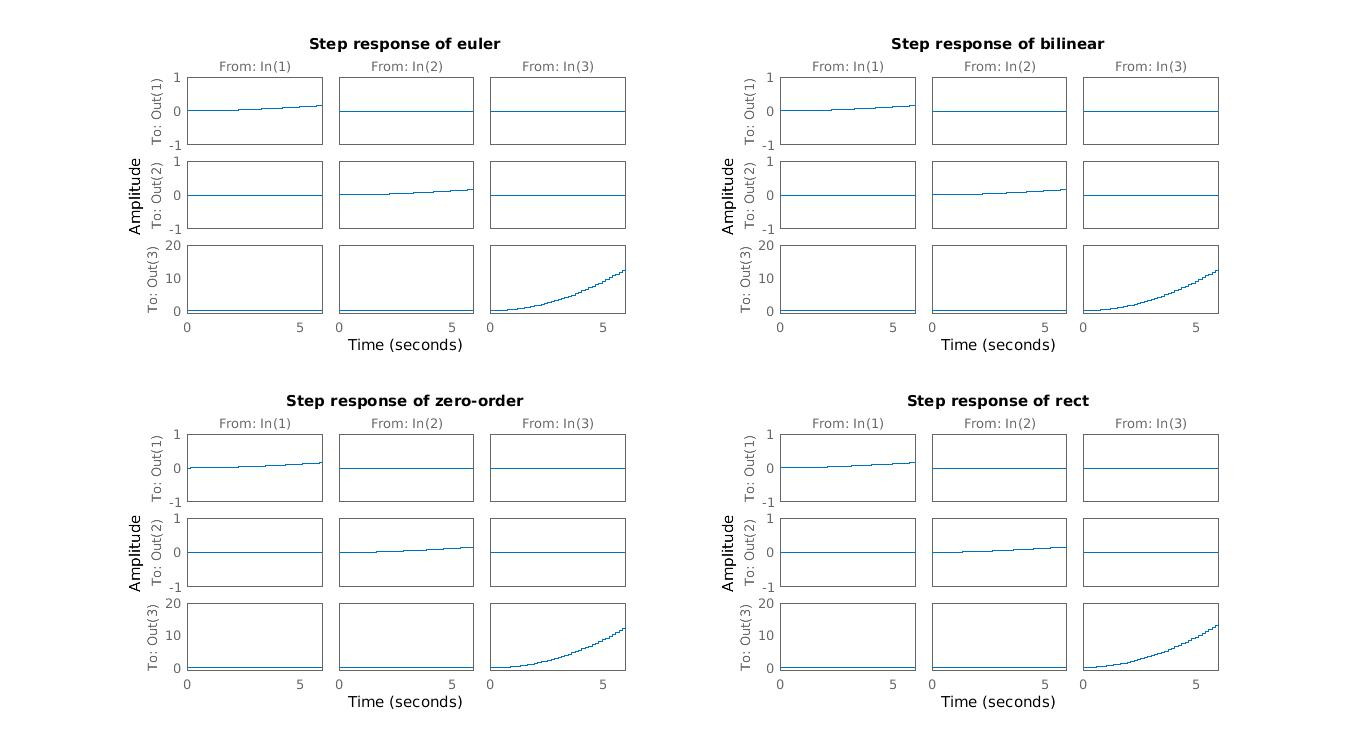
\includegraphics[width=\textwidth]{stepresponse.jpg}
\caption{Stepresponses of four discreted versions of the original model}
\end{figure}

\apicture{steprespcont.jpg}{Stepresponse of the continuous model}

\section{Setpoints}
The optimization problem exactly retrieves the input required to reach the reference states. The problem is however ill-conditioned, the matrix H used in the quadratic program has a condition number of $2.7006e+12$. Calculating the input with this matrix leads to the input sequence in the figure below on the left. We would like a smoother input and therefore we add a regularization term  $\mu \cdot I$ with $\mu$ a small number to H,  $\mu = 0.000001$ already gives a much better result. See the input on the right. 

\begin{figure}[H]
\begin{minipage}{.45\textwidth}
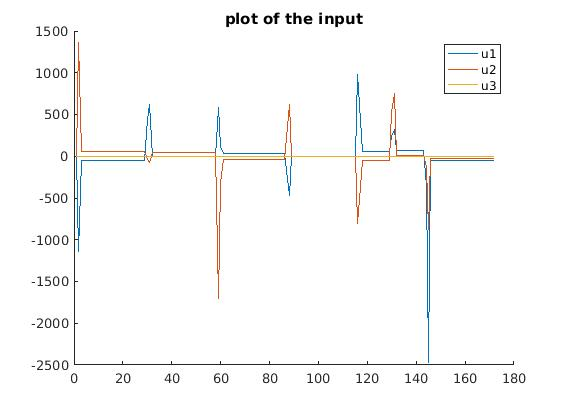
\includegraphics[width = \textwidth]{inputwithoutreg.jpg}
\end{minipage}
\begin{minipage}{.45\textwidth}
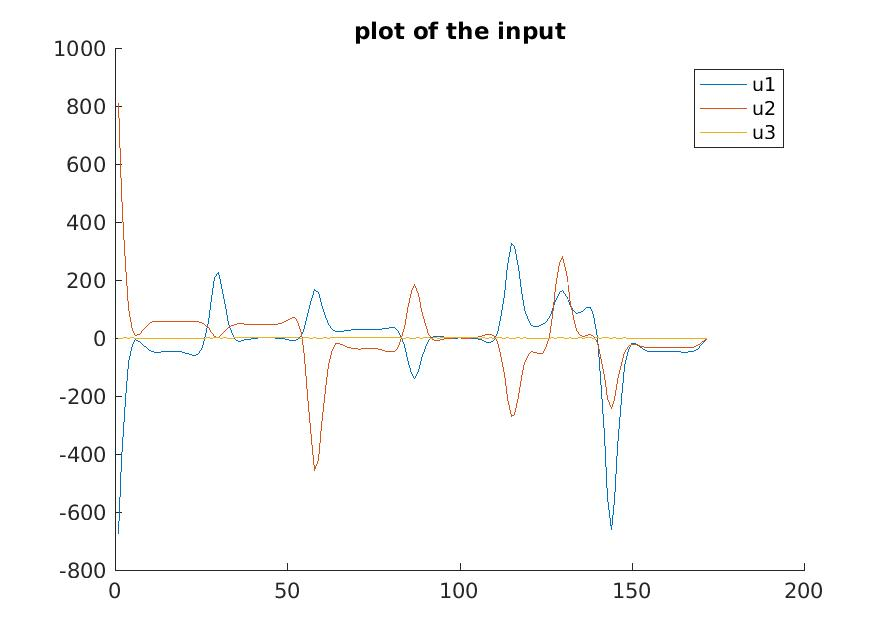
\includegraphics[width = \textwidth]{inputwithreg.jpg}
\end{minipage}
\caption{Optimal input calculated without and with a regularization term. For the input on the right the regularization term $\mu = 0.000001$}
\end{figure}

To calculate the reference state we simulate the system with our reference input. The figure below presents both the original reference path of the keeper and the newly calculated references.

\begin{figure}[H]
\centering
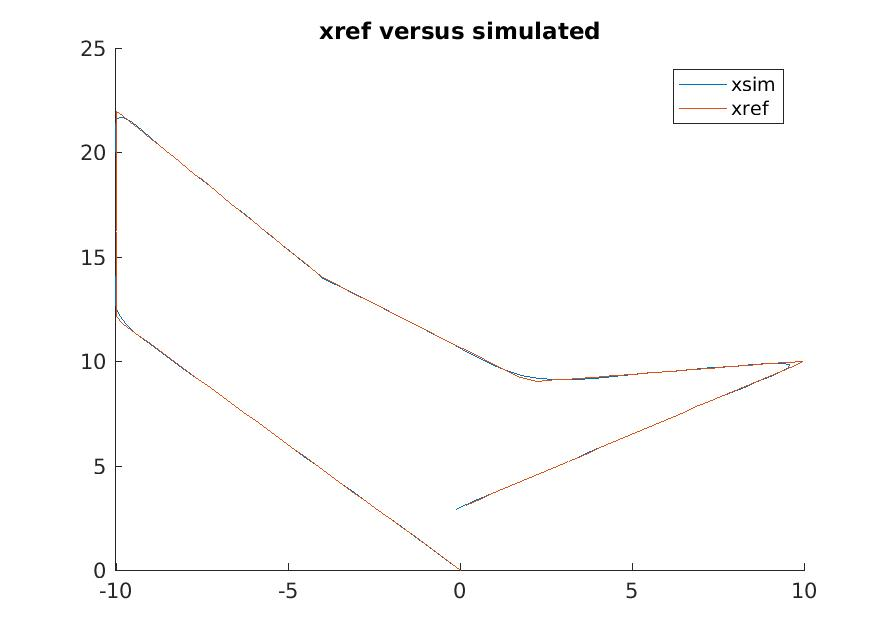
\includegraphics[width=.8\textwidth]{xrefstates.jpg}
\caption{Plot of original reference path and the newly calculated references}
\end{figure}

\section{LQR control}
We now are ready to control our keeper with LQR control. Two controllers were created according to the specifications, denoted $K_{lqr1}$ and $K_{lqr2}$. 
\begin{align*}
K_{lqr1} &= \left(\begin{array}{cccccc} 86.6 & 0 & 0 & 117.0 & 0 & 0\\ 0 & 86.6 & 0 & 0 & 117.0 & 0\\ 0 & 0 & 8.6 & 0 & 0 & 9.26 \end{array}\right) \\ K_{lqr2}&= \left(\begin{array}{cccccc} 89.9 & 0 & 0 & 89.4 & 0 & 0\\ 0 & 89.9 & 0 & 0 & 89.4 & 0\\ 0 & 0 & 38.9 & 0 & 0 & 7.92 \end{array}\right)
\end{align*}


In the figures below we subsequently plot the trajectories, the input signals and the states of both the controllers. 
\begin{figure}[H]
\begin{minipage}{.45\textwidth}
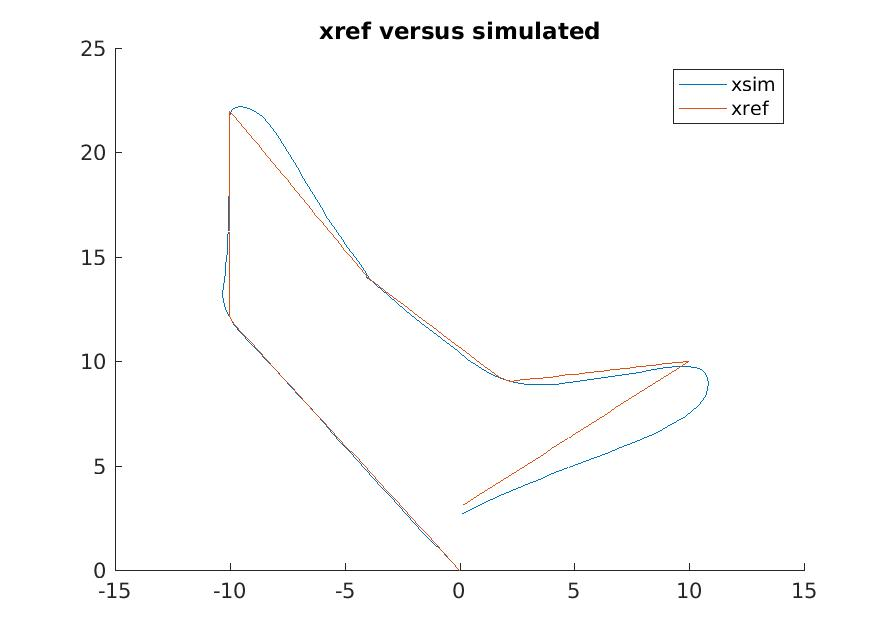
\includegraphics[width = \textwidth]{lqr1traj.jpg}
\end{minipage}
\begin{minipage}{.45\textwidth}
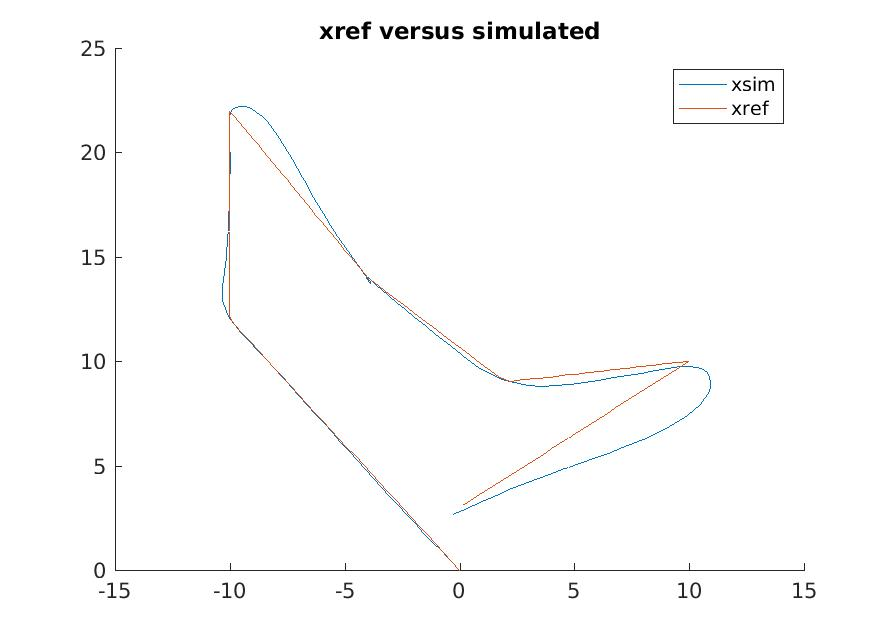
\includegraphics[width = \textwidth]{lqr2traj.jpg}
\end{minipage}
\caption{On the left the simulated trajectory with $K_{lqr1}$ and on the right $K_{lqr2}$ }
\end{figure}

\begin{figure}[H]
\begin{minipage}{.45\textwidth}
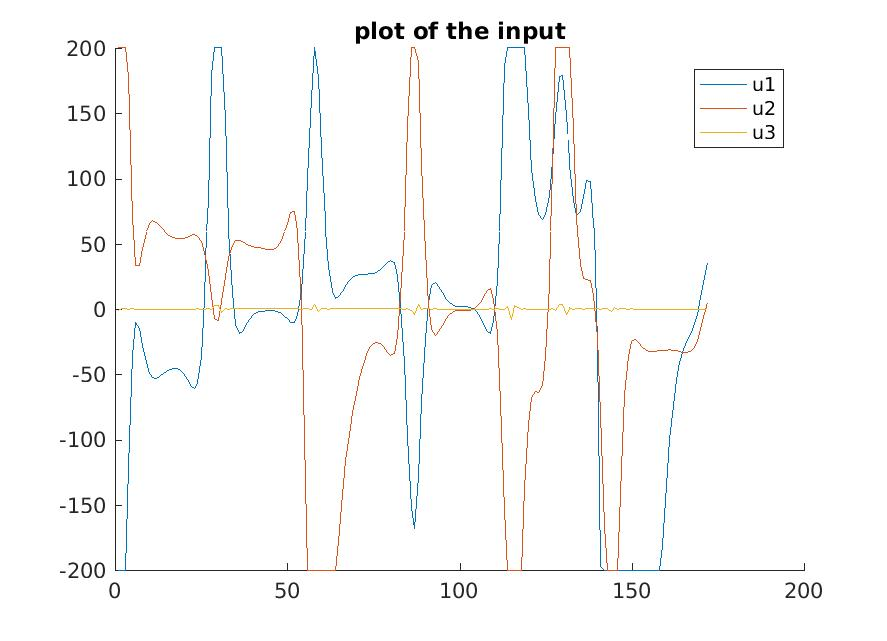
\includegraphics[width = \textwidth]{lqr1input.jpg}
\end{minipage}
\begin{minipage}{.45\textwidth}
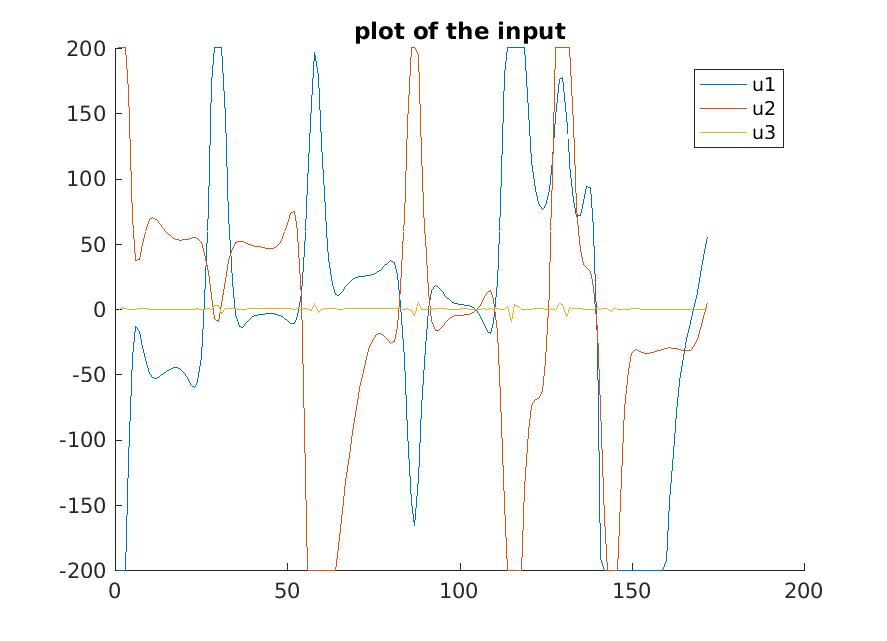
\includegraphics[width = \textwidth]{lqr2input.jpg}
\end{minipage}
\caption{On the left the input with $K_{lqr1}$ and on the right $K_{lqr2}$ }
\end{figure}

\begin{figure}[H]
\begin{minipage}{.45\textwidth}
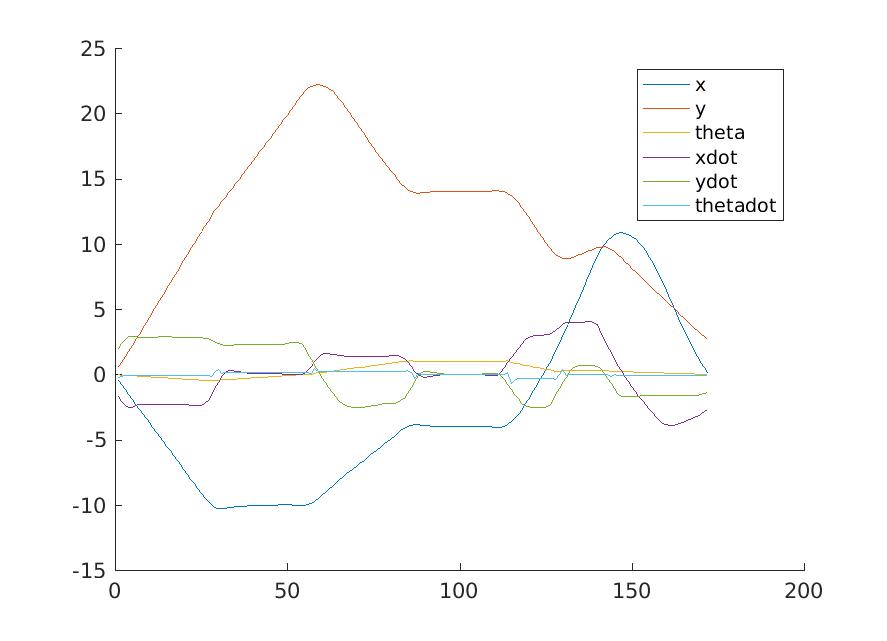
\includegraphics[width = \textwidth]{lqr1states.jpg}
\end{minipage}
\begin{minipage}{.45\textwidth}
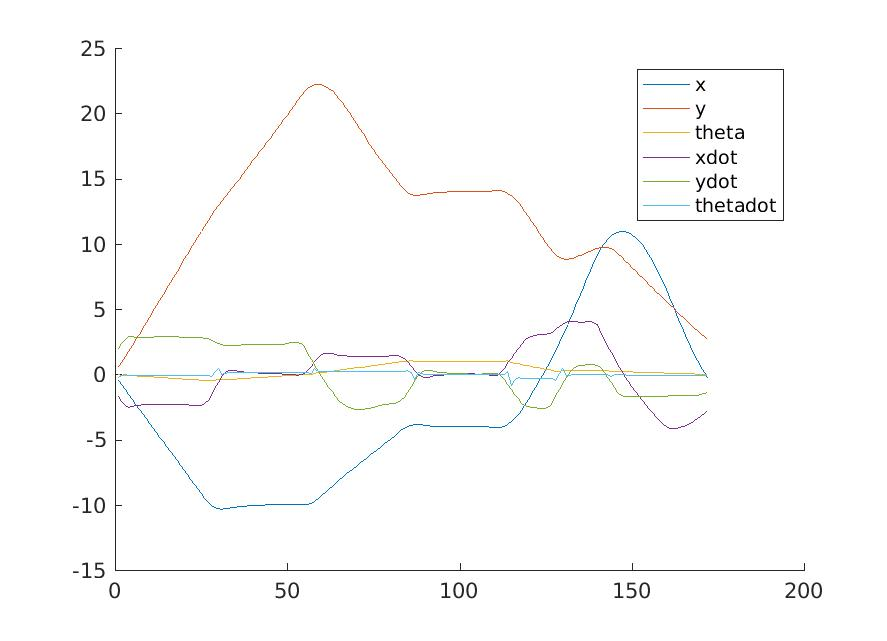
\includegraphics[width = \textwidth]{lqr2states.jpg}
\end{minipage}
\caption{On the left the sates of the simulated trajectory with $K_{lqr1}$ and on the right $K_{lqr2}$ }
\end{figure}

The cost of the simulation shows that the cost of the second controller is lower, namely 33.1349 versus 34.9471 respectively. The trajectories however look very similair. The fact that the plots are similair can be expected since the entries that were removed in the second controller mostly corresponds with disturbance rejection, and in our simulation there are no disturbances. 

\section{MPC}
Another approach we can take is that of the modelpredictive controller. Every timestep we will look ahead and calculate the subjectively "optimal" input to achieve the path closest to our reference states. The trajectory using a prediction horizon of 12 is shown below. 

\apicture{mpctraj12}{Simulate trajectory and the reference trajectory}

We also plot the control actions and the state variables, the simulation cost for a horizon of 12 is equal to 32.7179:

\begin{figure}[H]
\begin{minipage}{.45\textwidth}
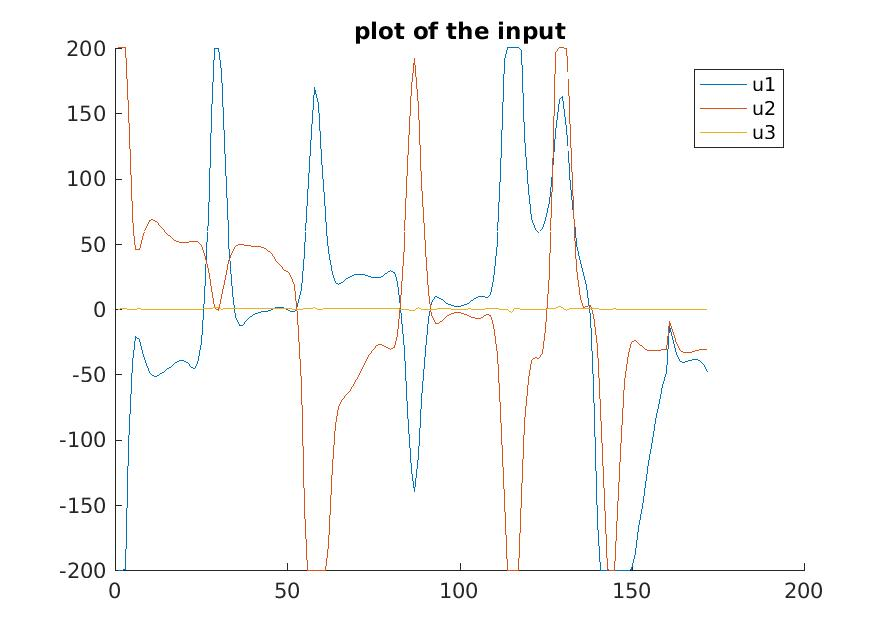
\includegraphics[width = \textwidth]{lqr1input12.jpg}
\end{minipage}
\begin{minipage}{.45\textwidth}
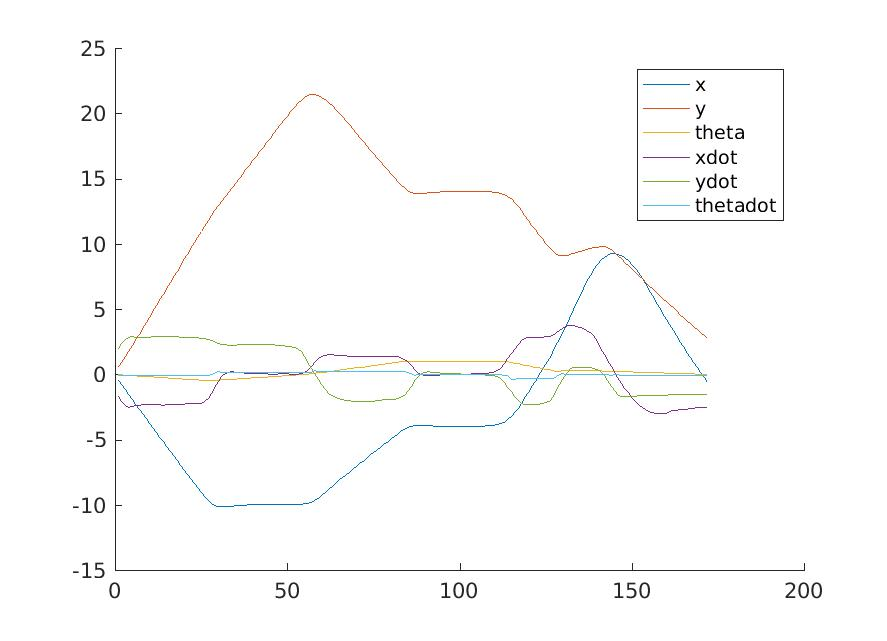
\includegraphics[width = \textwidth]{lqr1states12.jpg}
\end{minipage}
\caption{On the left control actions and on the right the states for an MPC controller with N = 12. }
\end{figure}



\end{document}